\subsection{Téléchargement}

    Pour télécharger le jeu, rendez vous sur la page https://lifeinvaders.github.io/website/, 
    et allez dans l'onglet télécharger. Cliquez ensuite sur l'icone correspondant à votre 
    système d'exploitation, et vous serez redirigé vers la page GitHub du launcher. 
    
    \begin{figure}[hbt!]
        \centering
        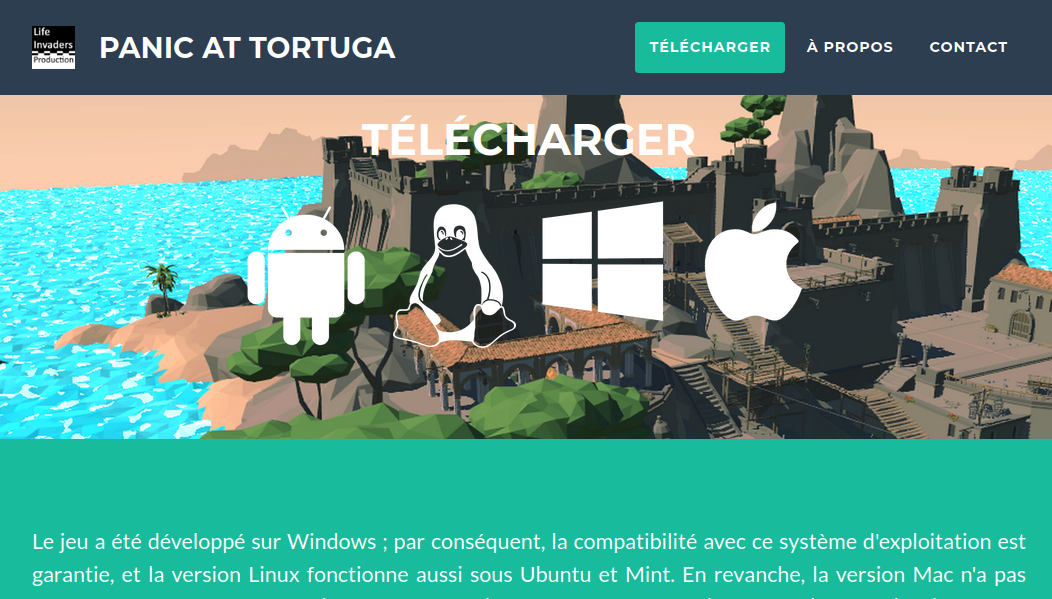
\includegraphics[scale=0.4]{img/dl_page.png}
        \caption{Page de téléchargement}
    \end{figure}
    \FloatBarrier
    

\subsection{Installation}

    Téléchargez-le, désarchivez-le 
    (à l'aide d'un logiciel comme 7zip par exemple), puis exécutez-le (il nécéssite les droits administrateurs, pour 
    installer pour tous les utilisateurs du poste). Une fois installé, le launcher apparaît dans le menu démarrer, et 
    sur le bureau si vous avez laissé cette option cochée.

    \begin{figure}[hbt!]
        \centering
        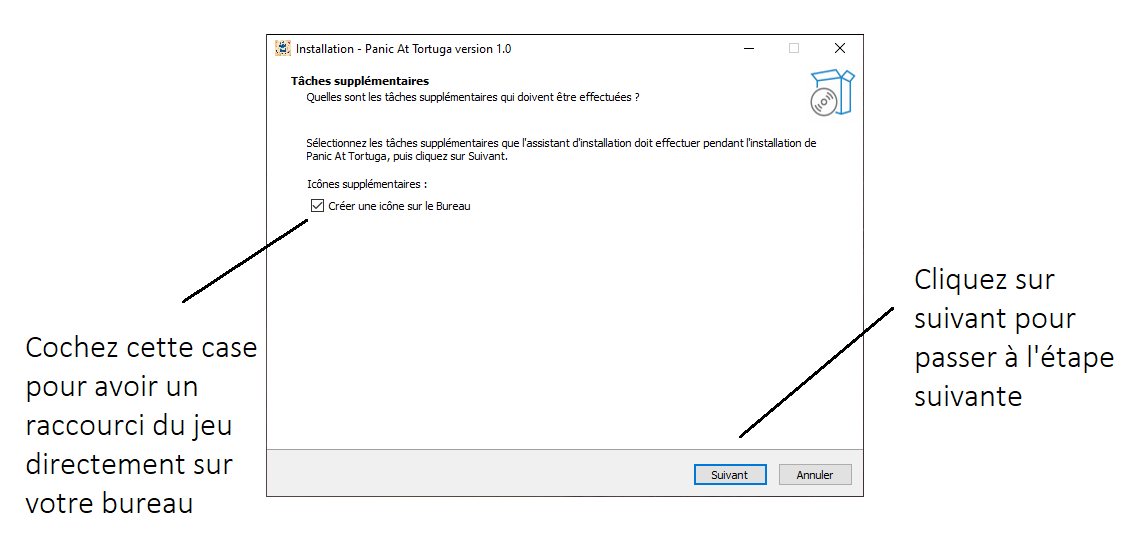
\includegraphics[scale=0.3]{setup_desktop.png}
        \caption{Ajout de l'icone sur le bureau}
    \end{figure}
    \FloatBarrier

    \begin{figure}[hbt!]
        \centering
        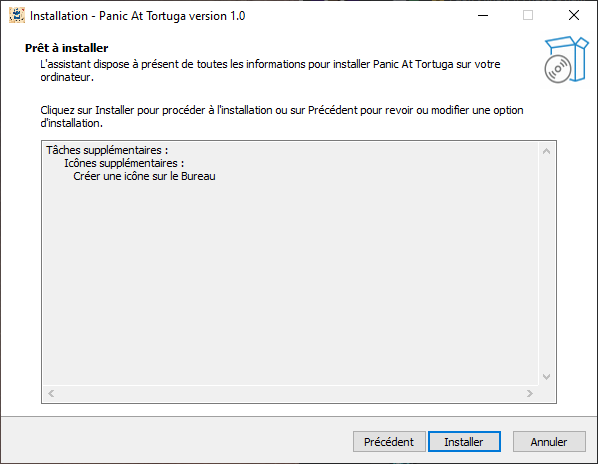
\includegraphics[scale=0.41]{setup_install.png}
        \caption{Installation du launcher}
    \end{figure}
    \FloatBarrier

    \begin{figure}[hbt!]
        \centering
        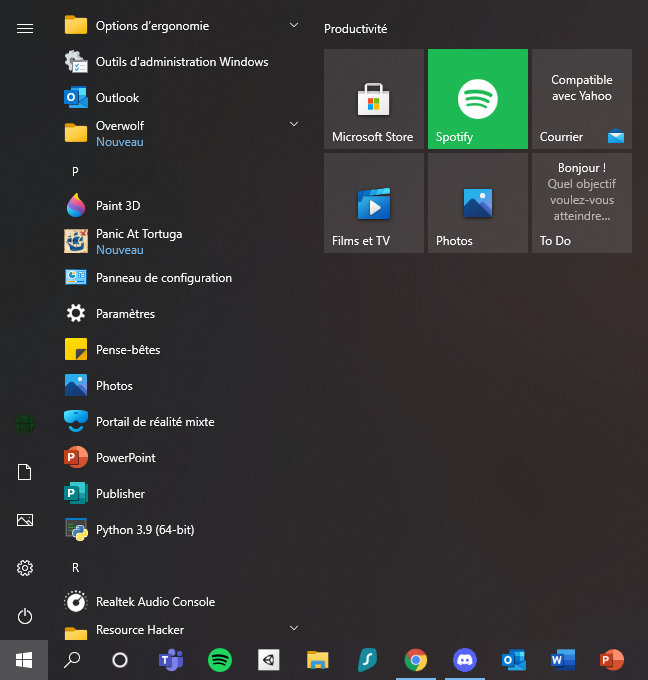
\includegraphics[scale=0.38]{start_menu.png}
        \caption{raccourci dans le menu Démarrer}
    \end{figure}
    \FloatBarrier

